%% ==============================
\chapter{Techniken der Dimensionsreduktion}
\label{ch:TechnikenDerDimRed}
%% ==============================


Hier werden ausgewählte traditionelle und moderne Techniken der Dimensionsreduktion vorgestellt.

\section{Traditionelle Methoden}
\label{ch:TechnikenDerDimRed:sec:TraditionelleMethoden}

Hier werden traditionelle Methoden vorgestellt.


\newpage

\subsection{Principal Component Analysis}
\label{ch:TechnikenDerDimRed:sec:TradtionelleMethoden:subsec:PCA}


\subsection{Kernel Principal Component Analysis}
\label{ch:TechnikenDerDimRed:sec:TradtionelleMethoden:subsec:kPCA}

\subsection{t-distributed Stochastic Neighborhood Embedding}
\label{ch:TechnikenDerDimRed:sec:TradtionelleMethoden:subsec:t-SNE}

\newpage


\section{Moderne Methoden}
\label{ch:TechnikenDerDimRed:sec:ModerneMethoden}

Hier werden Moderne Methoden vorgestellt.

\subsection{Autoencoder}
\label{ch:TechnikenDerDimRed:sec:ModerneMethoden:subsec:AE}

\begin{figure}[h]
  \begin{center}
    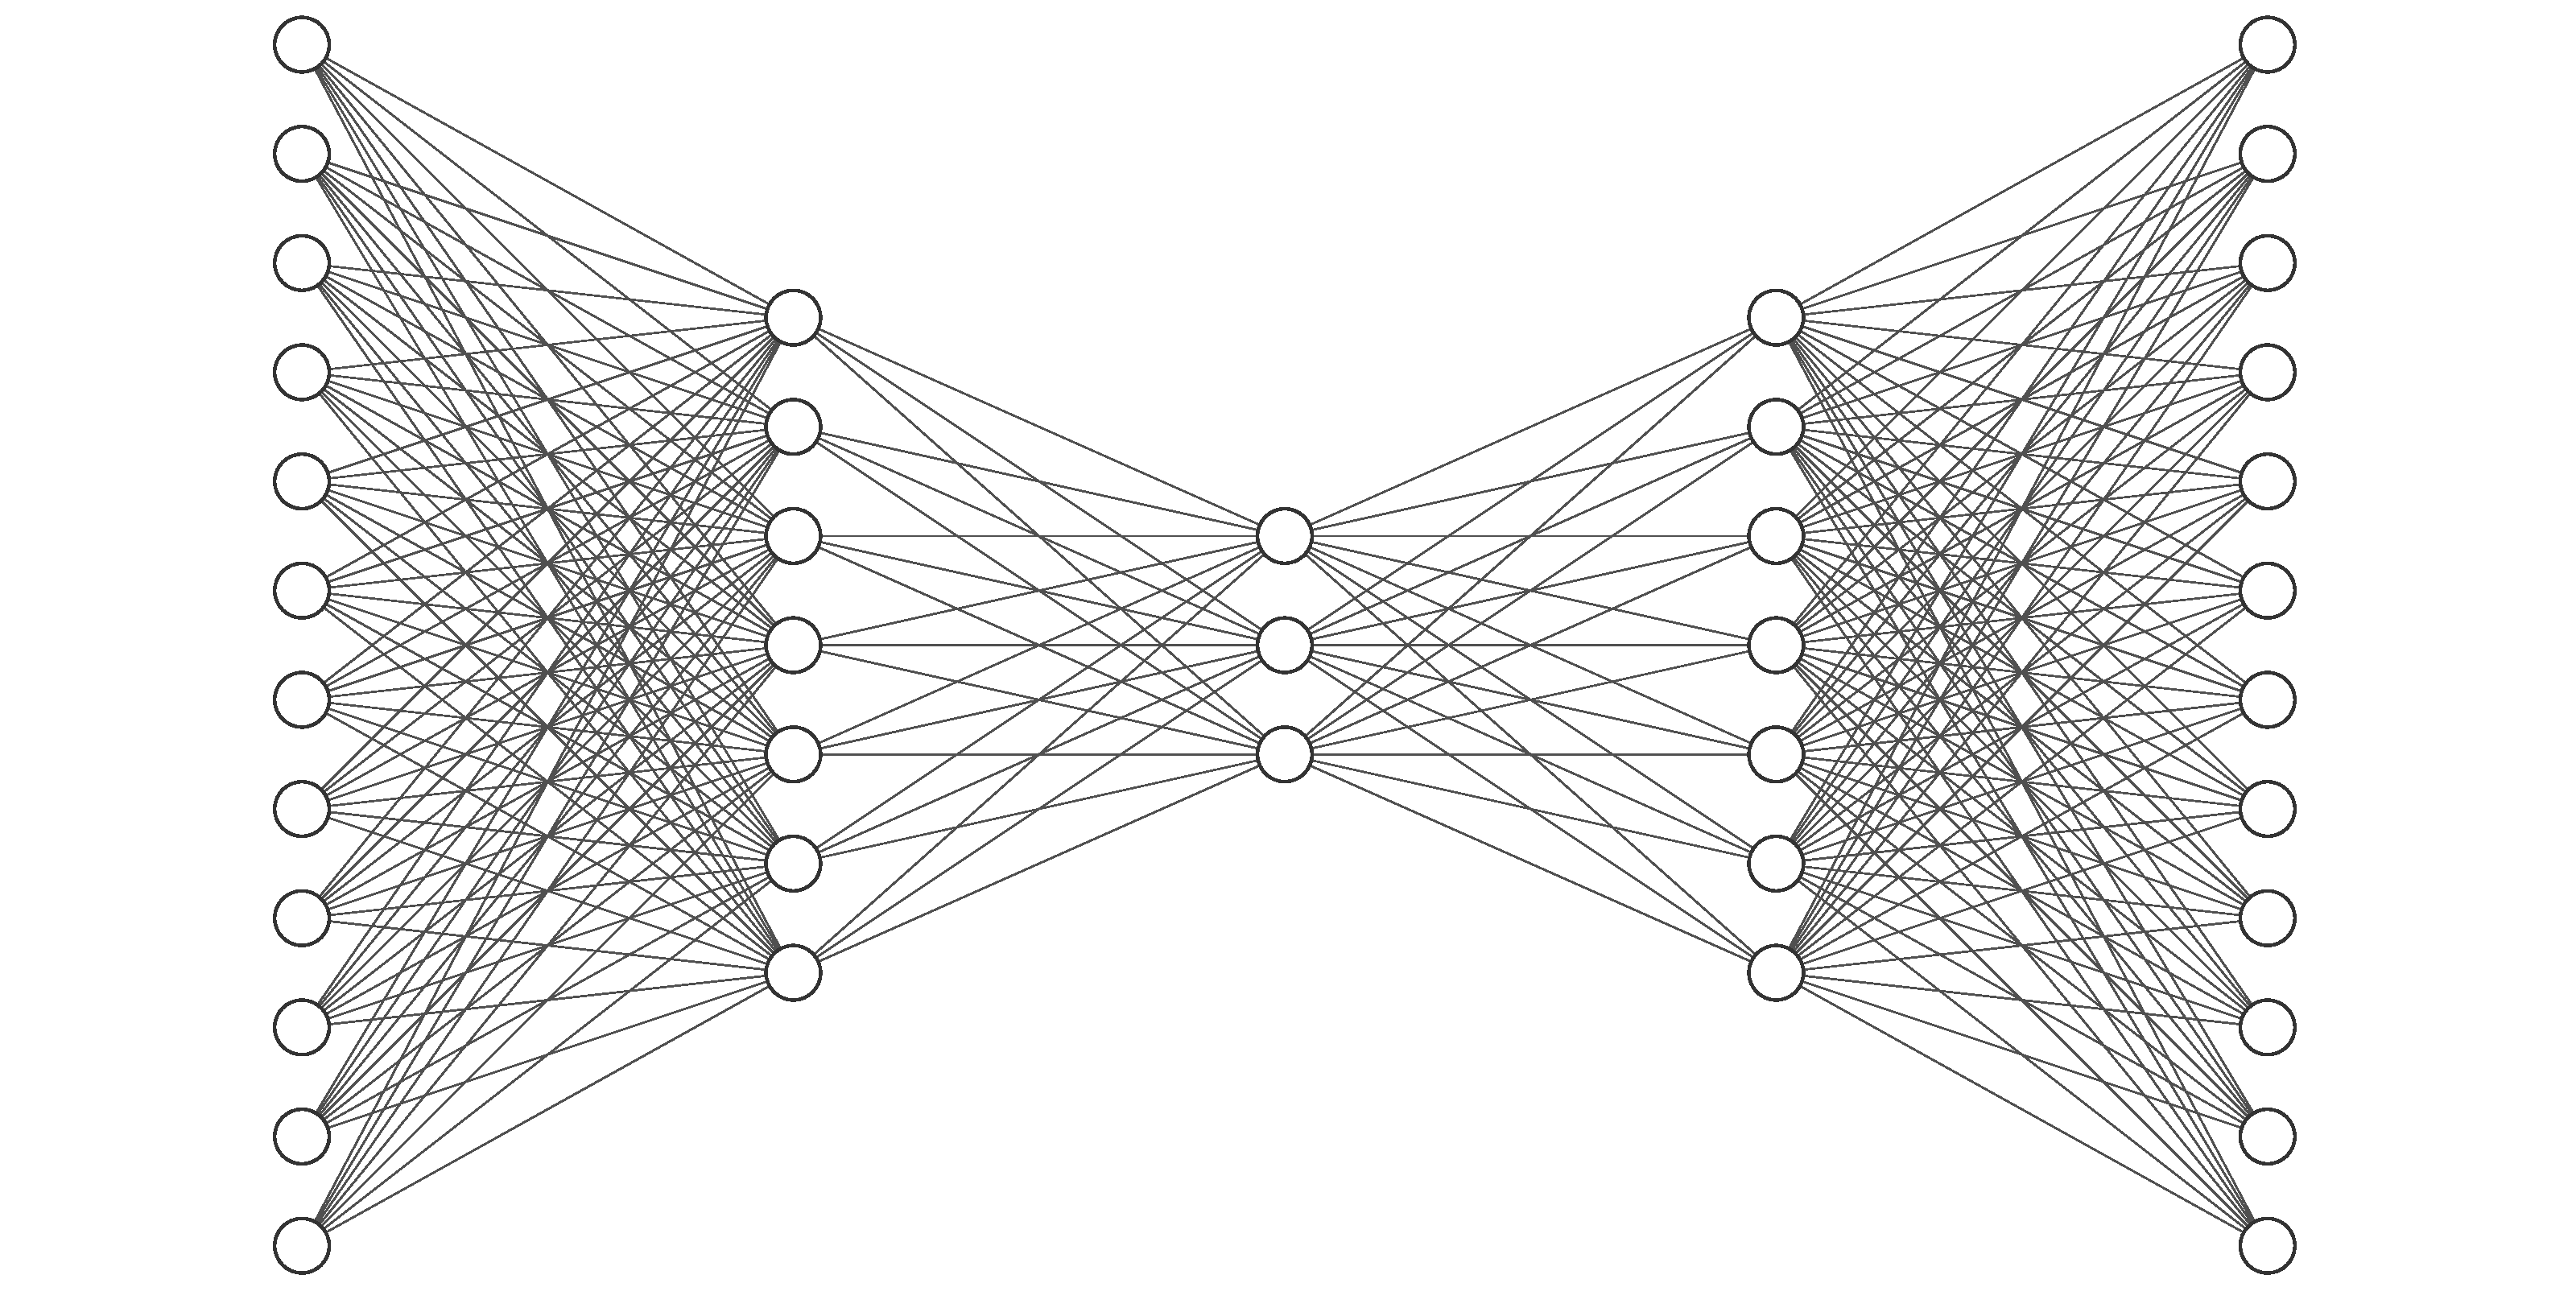
\includegraphics[width=\textwidth]{5_layer_AE.pdf}
    \caption{Autoencoder mit fünf Schichten und dreidimensionalem Bottleneck.}
  \end{center}
\end{figure}

\subsection{Variational Autoencoder}
\label{ch:TechnikenDerDimRed:sec:ModerneMethoden:subsec:VAE}

\subsection{Self-Organizing Maps}
\label{ch:TechnikenDerDimRed:sec:ModerneMethoden:subsec:SOM}
